\documentclass[12pt,a4paper]{article}
\usepackage{CJKutf8}
\usepackage{enumerate}
\usepackage{color}
\usepackage{graphicx}
\usepackage{indentfirst}
\usepackage{multirow}
\graphicspath{{./img/}}
\title{{\Huge{YokeEmulator}} \\1.1.0.0 Manual}
\author{SxS\footnote{email:shinesong\_sxs@foxmail.com QQGroup:303579244}}
\begin{document}
\begin{CJK}{UTF8}{gbsn}
\maketitle
\newpage
\tableofcontents

\newpage
\section{Introduction}
\subsection{YokeEmulator WP}
YokeEmulator(WP) is a Joystick \& header tracker mobile App,to use that you should have \textbf{YokeEmulator Server} \textbf{OpenTrack} and \textbf{vJoy}
\subsection{YokeEmulator Server}
YokeEmulator is a upper computer run on your PC, receive your mobile sensor signal and send to Game.It's an essential suite for YokeEmulator.
\subsection{vJoy}
vJoy is a device driver that bridges the gap between any device that is not a joystick and an application that requires a joystick. If you develop an application for windows that requires user physical input you should consider incorporating vJoy into your product.


vJoy can be incorporated as-is or modified. vJoy can be used with fixed configuration or configurable. It also comes with tools and example code that feeds it with data and configure the virtual joystick.


vJoy is implemented as a joystick virtual-device driver for windows (XP and up) that does not represent an actual hardware device.


The vJoy device is seen by Windows as a standard joystick device. However, it receives its signals through a simple software interface. Coders can take advantage of this interface by modifying the provided sample code.


\textbf{Download} : http://vjoystick.sourceforge.net/site/index.php/download-a-install
\subsection{Opentrack}
Opentrack is an application dedicated to tracking user's head movements and relaying the information to games and flight simulation software.


Not to be confused with railway planning software <http://opentrack.ch>


\textbf{Home Page} : https://github.com/opentrack/opentrack
\newpage
\section{Installation}
\begin{enumerate}[\textbf{Step} 1.]
\item Install vJoy 2.0.5.
\\*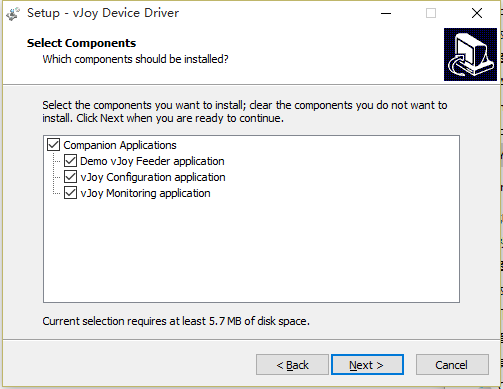
\includegraphics[width=4in]{install_vjoy.png}
\item Config vJoy use vJoyConf.
\\*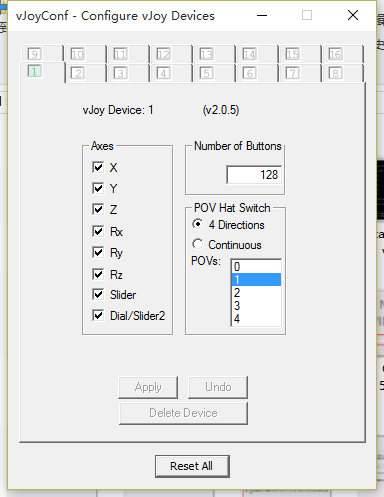
\includegraphics[width=4in]{install_config_vjoy.png}
\item Test vJoy use vJoy Moniter and Feeder Demo.
\\*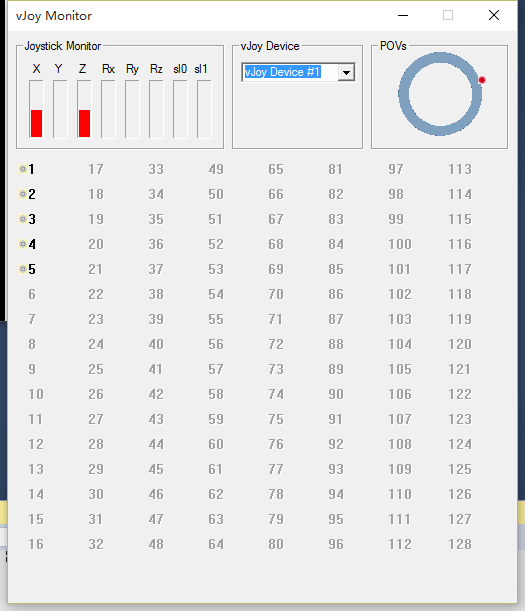
\includegraphics[width=4in]{install_test_yoke.png}
\item Download and uncompress OpenTrack package,then run \textbf{opentrack.exe}.
\\*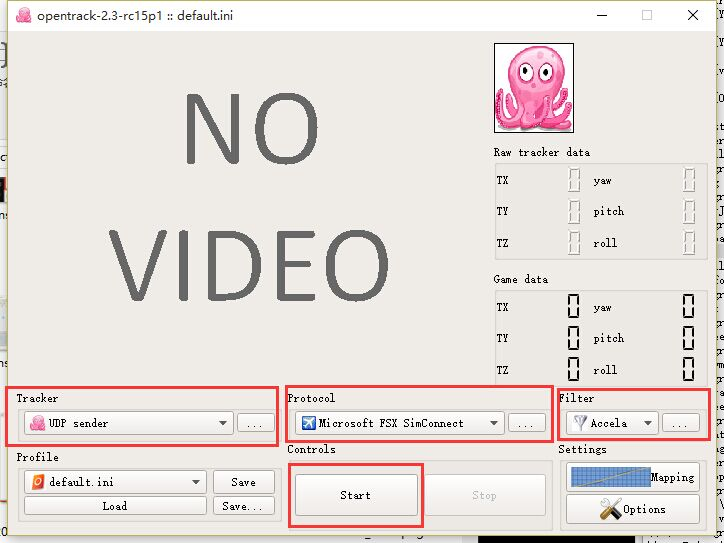
\includegraphics[width=4in]{install_opentrack.jpg}
\\Set \textbf{Tracker} to \textbf{UDP sender},and check the config port.Set protocol according to your game.Set \textbf{Filter} to \textbf{Accela} as recommend,finally Press \textbf{Start} button.
\item Install .Net framework 4.5.2.
\item Test for YokeEmulatorServer,Like this
\\*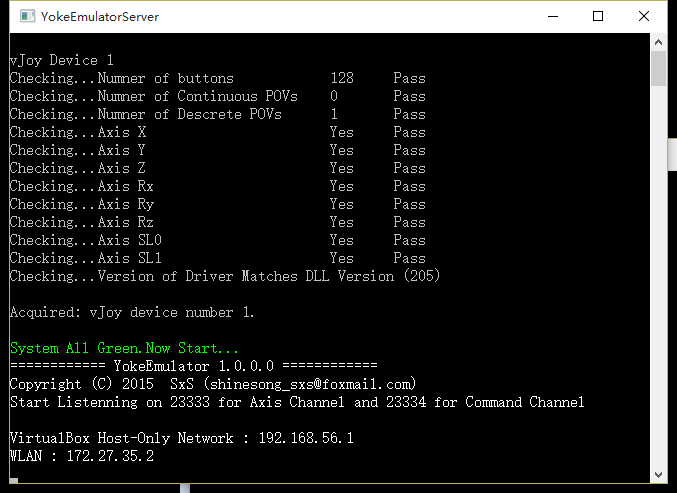
\includegraphics[width=4in]{install_finish_server.png}
\item Unlock your phone with your Developer MS Account,use \textbf{Windows Phone Developer Registration 8.1}
\\*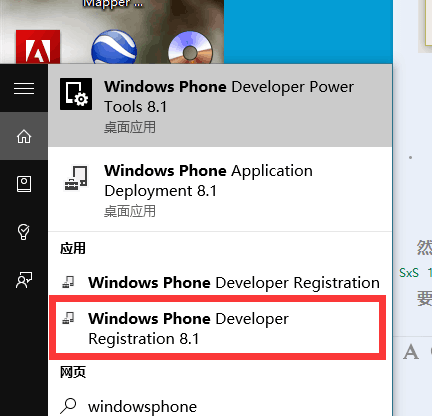
\includegraphics[width=4in]{install_registration_phone.png}
\\*If you see this message,your phone is already unlocked.Like this.
\\*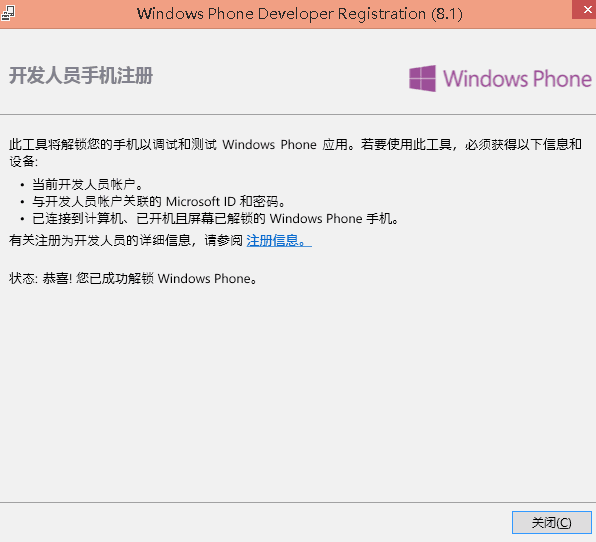
\includegraphics[width=4in]{install_unlock_success.png}
\item Deployment App to your phone.
\\*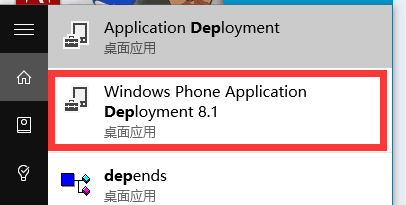
\includegraphics[width=4in]{install_deploy.png}
\\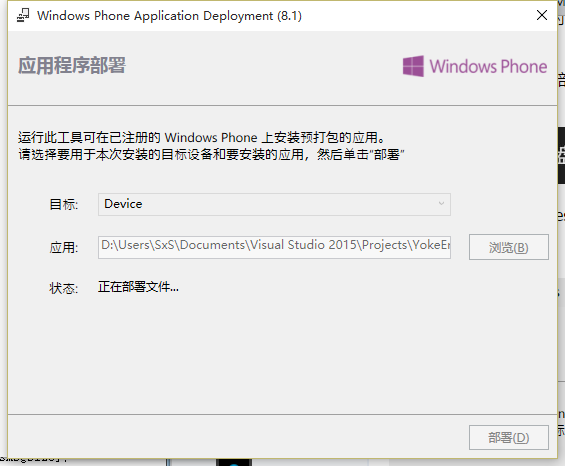
\includegraphics[width=4in]{install_deployment.png}
\\*If you see this message,you have deploy app success.
\\*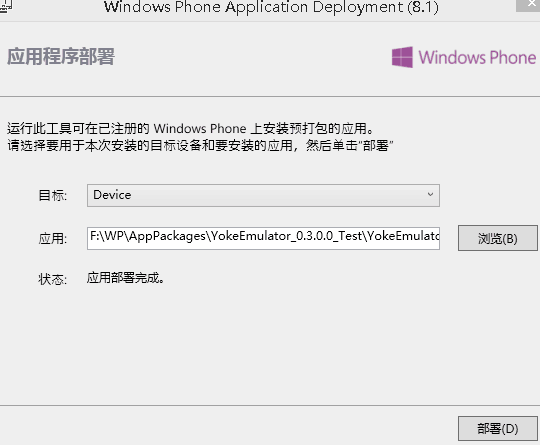
\includegraphics[width=4in]{install_deployment_success.png}
\end{enumerate}

\newpage
\section{Usage}
\begin{enumerate}[\textbf{Step} 1.]
\item Make sure your phone connect to WiFi which can access to your pc.
\item Run Opentrack and press Start button for HeadTracker.
\item Run YokeEmulator Server, you can read avaliable ip and interface name from newest message.
\\*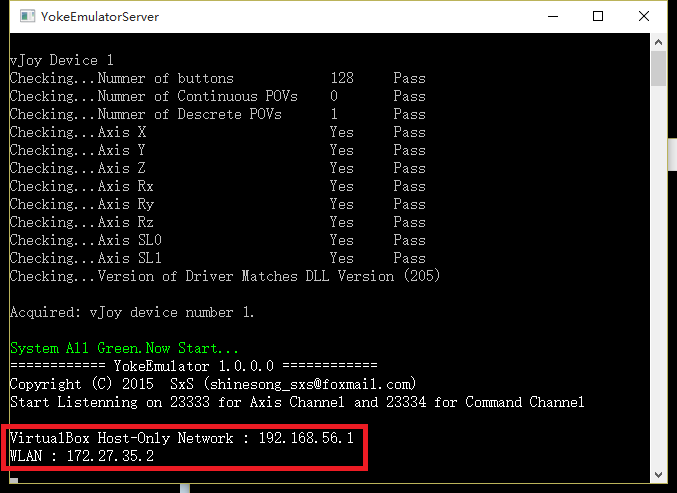
\includegraphics[width=4in]{usage_runserver.png}
\item Run YokeEmulator App on your phone,you can see main page like this.
\\*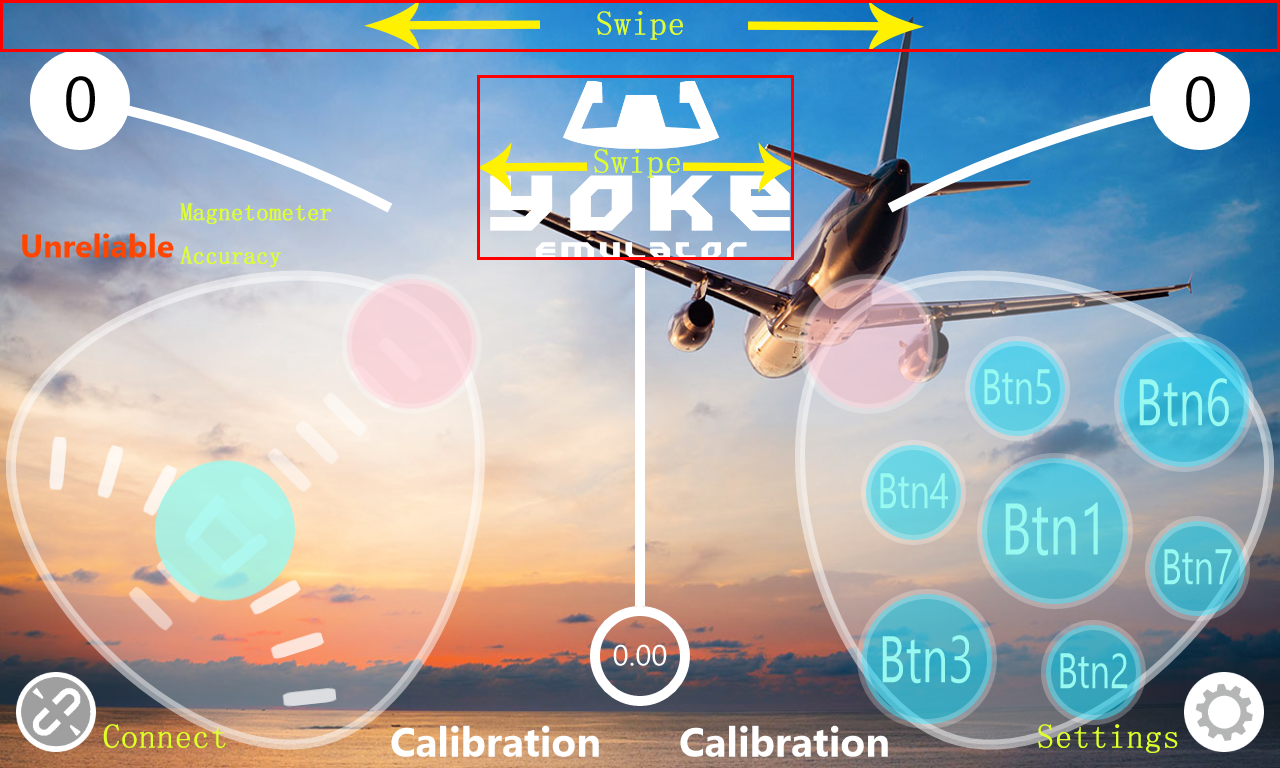
\includegraphics[width=4in]{usage_controlArea.png}
\\This page have two Buttons,in left bottom and right bottom corner.The top long red box area is \textbf{Page Swithcer},you can swipe left and right switch to other page.Also,you can swipe horizonal on Logo Area to switch sensor mode,include \{None,Joystick,Tracker\}.
\item Press setting button on the right bottom corner to navigate to \textbf{Settings Page}.You can set pc IP, opentrack port and other fucntions here.
\\*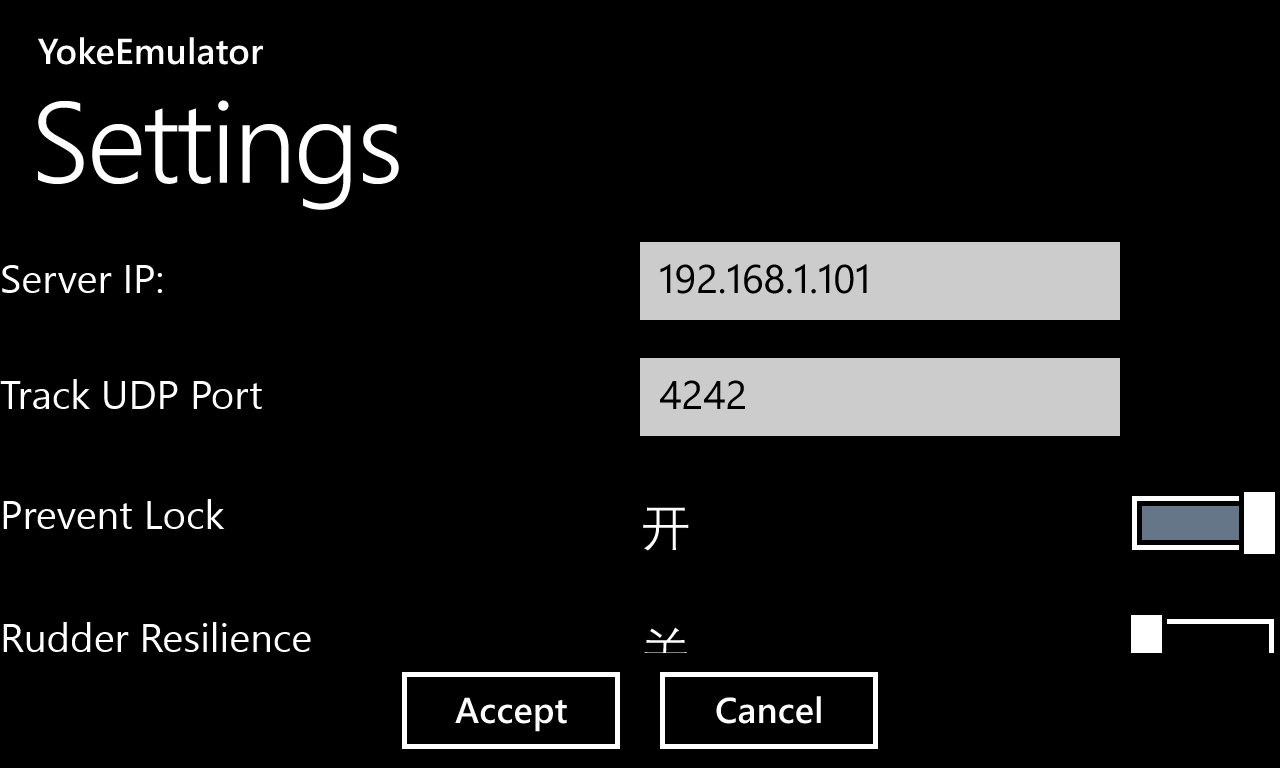
\includegraphics[width=4in]{usage_settings.png}
\\When you finish edit,press \textbf{Apply} to save changed.
\item Press \textbf{Connect} button on the left-bottom of screen.
\item You can use Page Switcher navigate to another page,called BattlePage.
\\*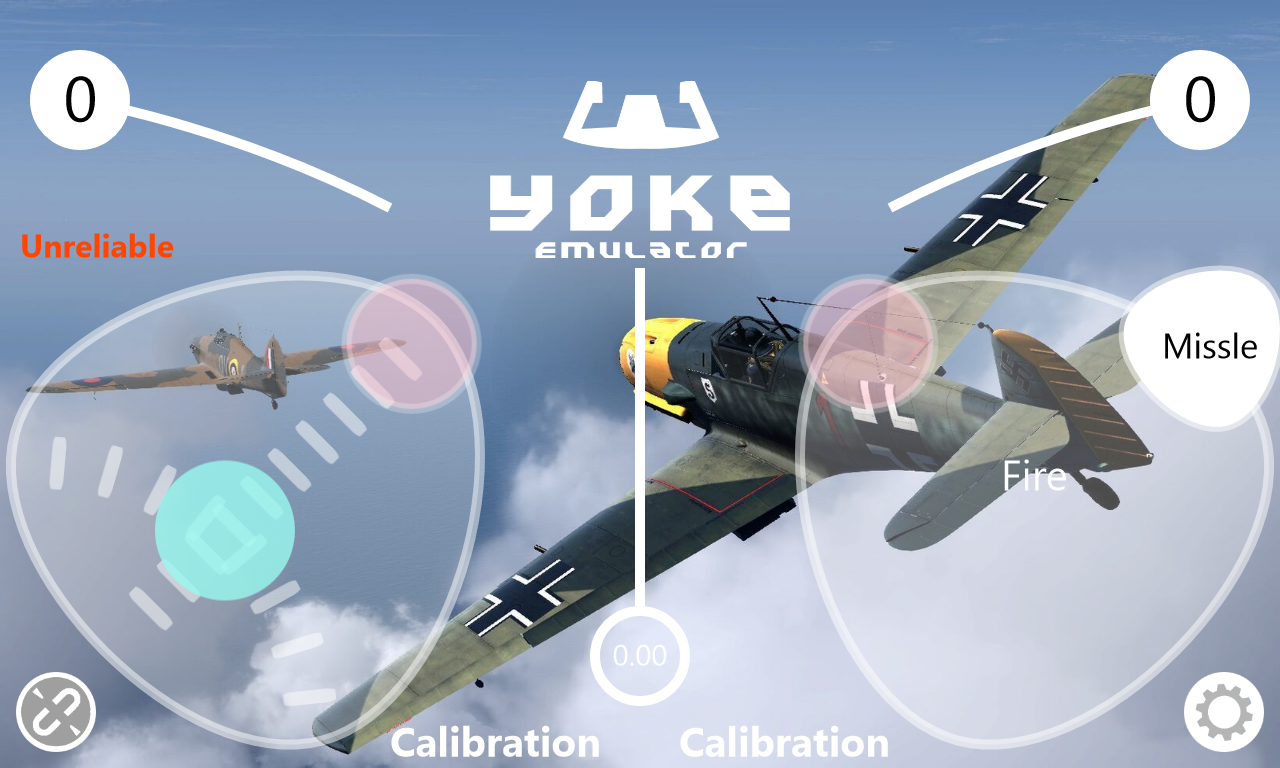
\includegraphics[width=4in]{useage_battlepage.png}
\item The left pad is called Rudder Pad,and the right is called Button Panel.They both have a red point on the corner,it's called Tracker Trigger, you may pressed both of them together to active Tracker Mode.And when you release both of them, mode will return to normal.
\item You can press two red point, and move your finger up and down to opposite direction,you can zoom the viewport,experiment yourself.
\item You can see two Calibration label on the center-bottom of page,when you press both of them, program is setting to Calirating mode,when you release them.The attribute of your phone will be record as normal attribute.
\end{enumerate}

\newpage
\section{Develope}
\subsection{YokeEmulatorServer Protocol}
YokeEmulator Server Listen at two udp channel,port is \textbf{23333} (joystick axis) and \textbf{23334} (ctrl commmand).You can send message to these port act as joystick.\\
\begin{center}
\textbf{JoyStick Axis Protocol}\\
\begin{tabular}{c|c|c}
\hline \textbf{bit} & \textbf{type} & \textbf{Comment} \\
\hline 0-7 & double & X-axis value (0-1) \\
\hline 8-15 & double & Y-axis value (0-1) \\
\hline
\end{tabular}
\end{center}

\begin{center}
\textbf{Control Command Protocol} \\
\begin{tabular}{c|c|c}
\hline \textbf{bit} & \textbf{type} & \textbf{Comment} \\
\hline 0 & char & op flag\\
\hline 1-8 & double or char*2+blank & value or [bid][state]+[0]*6 \\
\hline
\end{tabular}
\end{center}

\textbf{Note:} flag \{'x','y','z','X','Y','Z','s','l'\} for 8-axis 'b' for button 'p' for POV, when op is axis flag(XYZ correspond for rx,ry,rz),value should be 0-1;when op is 'p', value should be 0-360\&-1(empty);when op is 'b',only first two bytes are avaliable,bid represent button id (1-128),state is an binary value(0 for released,1 for pressed). \\
\subsection{Opentrack UDP Receiver Protocol}
\begin{center}
\textbf{Control Command Protocol} \\
\begin{tabular}{c|c|c}
\hline \textbf{bit} & \textbf{type} & \textbf{Comment} \\
\hline 0-7 & char & tx\\
\hline 8-16 & double & ty \\
\hline 17-24 & double & tz \\
\hline 25-32 & double & yaw \\
\hline 33-40 & double & pitch \\
\hline 41-48 & double & roll \\
\hline
\end{tabular}\end{center}
\section{ChangeLog}
\subsection{1.1.0.0}
\begin{enumerate}
	\item Add two Axis to main page.
	\item Support most to 3-axis 1-rudder 7/2 buttons,joystick and headtracker.This is a stable version.
\end{enumerate}
\subsection{1.0.0.0}
\begin{enumerate}
	\item Change UI presentation.Make it comfortable for manipulating.
	\item Reconstruct App to provide powerful handling.
	\item Add battle Page
	\item Add Header Tracker Zoom
	\item Add Calibration
	\item Add Gesture manipulation.
\end{enumerate}
\subsection{0.3.0.0}
\begin{enumerate}
	\item Add Head Tracker mode.
\end{enumerate}
\subsection{0.2.0.0}
\begin{enumerate}
	\item Support for X Y Axis,Z for Rudder Axis,Slider Axis.Up to 128 buttons/toggle.Swithable Discrete 4 director Hat/Continual Hat;
	\item Customize Button/Toggle,Buttons Name;(See Settings page)
	\item Keep Screen unlock;
\end{enumerate}
\subsection{0.1.0.0}
\begin{enumerate}
	\item Support for X Y Axis,Slider Axis,4 buttons and Continual Hat;
\end{enumerate}
dev
\end{CJK}
\end{document}
